%____________________________________________________________________________
%
% author: Januario Carreiro <jjc70@duke.edu>
% created: 7 March 2020
%____________________________________________________________________________
\documentclass[12pt]{../manual} 
%____________________________________________________________________________
%
%	TITLE AND TABLE OF CONTENTS
%____________________________________________________________________________
\begin{document}
\makeheader{Lab 5}
\begin{center}
\textbf{\huge ECE 230L - LAB 5 Solution}\\~\\
\textbf{\large Signal Transmission}\\~\\
\rule{6.5in}{0.5mm}\\
\end{center}

\tableofcontents

\listoffigures
%____________________________________________________________________________
%
%	BODY
%____________________________________________________________________________
\newpage

\section{Music Transmitter}
\subsection{Order of Components}
\begin{figure}[ht!]
\centering
\begin{circuitikz}
\draw (0,0)		to[R, a=$R_4$, *-] ++(0,3)
				to[pR, a=$P_1$, name=P] ++(0,3)
				to[R, a=$R_3$] ++(0,3)
				to[short, *-] ++(-12,0)
				to[battery, l=$V_S$, a=\SI{9}{\volt}] ++(0,-9)
				to[short] ++(15,0);
\draw (3,4.5) node[nigfete, solderdot, name=N]{};
\draw (N) circle [radius=25pt];
\draw ($(N) + (0.9,0)$) node[right] {BS170};
\draw ($(N.S) + (0,0.2)$) 	to[short,*-] ++(0.5,0)
							to[zzD*,diodes/scale=0.3] ++(0,1.15)
							to[short, -*] ++(-0.5,0);
\draw (0,9)		to[short] ++(3,0)
				to[R, a=$R_5$] ++(0,-3) -- (N.D);
\draw (N.S) -- (3,3) to[leD*, a=$D_1$] ++(0,-3);
\draw (-8,0)	to[short, *-] ++(0, 1.5)
				to[R, a=$R_1$] ++(0,3)
				to[C, a=$C_1$, v^<=$~$] ++(3,0)
				to[R, a=$R_2$] ++(3,0) -- (P.wiper);
\draw (-1.5,4.5)to[short, *-] ++(0,1.5)
				to[xing] ++(3,0) |- (N.G);
\draw (-8,1.5)	to[short, *-o] ++(-1,0);
\draw (-8,4.5)	to[short, *-o] ++(-1,0);
\draw (-9,4)	node[] {$+$};
\draw (-9,2)	node[] {$-$};
\draw[red,thin,dashed] (-10.5,5) rectangle (-8.5,1);
\draw (-9.5,3.25) node[] {$1/8$''};
\draw (-9.5,2.75) node[] {mini plug};
\end{circuitikz}
\caption{Music Transmitter Circuit}
\end{figure}

\subsection{Reasoning Behind Order of Components}
The components, $R_5$, $D_1$, and the BS170 can go in any order you choose. The infrared diode is controlled by current. Current can only flow through the path consisting of the $R_5$, $D_1$, and the BS170 when a positive voltage is applied to the gate of the BS170. Further, while the MOSFET controls whether the current is on or off, $R_5$ controls how much current is flowing through the path (remember, $V=IR$). Since the current in a path is the same throughout the entirety of the path, the resistor can be placed both before and after the infrared diode.

\newpage
\section{Wireless Transmission with M1K}
Output of M1K to be added soon.
\begin{figure}[ht!]
\begin{center}
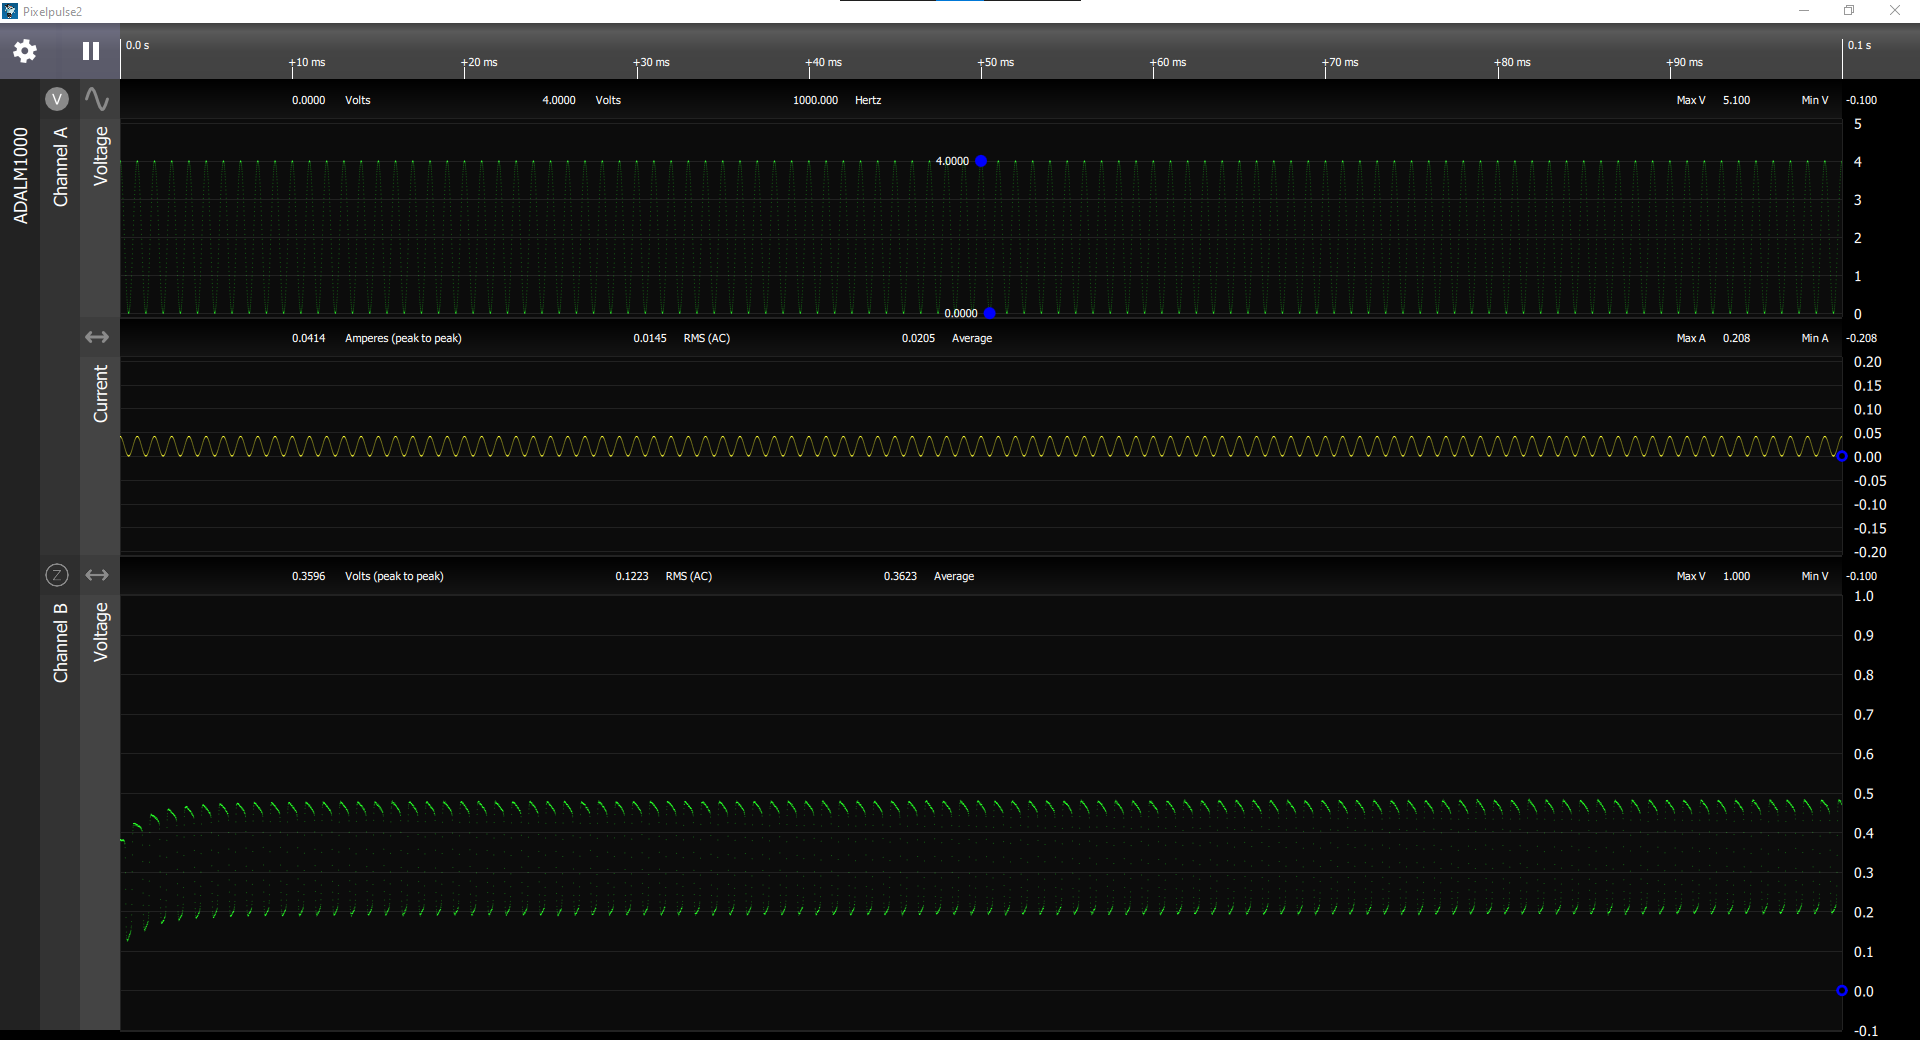
\includegraphics[width=\textwidth]{figures/M1KSolution}
\end{center}
\end{figure}

\newpage
\section{Question 1}
\textit{In lab, the BS170 MOSFET is used. Define the parameters $K_N$ and the transconductance $g_m^\mathrm{sat}$ of the NMOSFET. Comment on their dependence on other NMOSFET parameters and bias voltages.}

$K_N$ is the ``conductance parameter'' and depends on the geometry of the MOSFET (channel width, channel length, capacitance oxide, etc.).
\begin{align}
K_N = \frac{\mu_N^{ch}C_{ox}W_{ch}}{L_{ch}}
\end{align}
$g_m^{sat}$ is the forward transconductance in the saturation bias range. It depends on a lot of the same parameters as $K_N$ as well as the MOSFET's bias voltages.
\begin{align}
g_m^{sat} = K_N \left( V_{GS} - V_{TN}(V_{BS}) \right)
\end{align}
We will also accept
\begin{align}
g_m^{sat} = K_N \left( V_{GS} - V_{TN} \right).
\end{align}
\section{Question 2}
\textit{In lab, the LM 86 op-amp is used. In general, why are op-amps used in circuits? In the case of the LM386 specifically, what is the gain? Can this value be changed? If so, how? Also, what kinds of loads can this op-amp drive?}

An operational amplifier, or an op-amp, is used when a higher voltage difference is necessary. It produces an output potential that is a multiple of the difference between its input terminals. The LM386 op-amp has a gain of 20 when there is no capacitor between pins 1 and 8. The gain can thus be changed from any value between 20 and 200 depending on the capacitance of the capacitor placed between pins 1 and 8. In lab, the LM386 has a gain of 200. The LM386 can drive loads from \SI{4}{\ohm} to \SI{32}{\ohm}.
\section{Question 3}
\textit{How can one improve the quality of the receiver circuit? Would placing a capacitor between power and ground improve or worsen the quality? Why?}

Yes, placing a capacitor between power and ground would improve quality by acting as a resorvoir for the op-amp when it rails (i.e. when output voltage gets close to $V_S$).

\newpage
\section{Question 4}
\textit{Why do we set the M1K to produce a signal between \SI{20}{\hertz} and \SI{20}{\kilo\hertz}? Do we have to change the resistance of the potentiometer based on whether we are in the lower range or upper range of that bound?}

We set the M1K to produce a signal in that range because that is the human hearing range. That's the range that will allow us to hear whether the circuit is working.

We do not have to change the resistance of the potentiometer based on whether we are in the lower or upper range of that bound because changing the resistance of the potentiometer will only change the amount of current going through the path with the potentiometer and the path with the diode. Once the potentiometer is set to a resistance value that results in a close-to-optimal amount of current flowing through the diode, a signal of any reasonable frequency will be able to transmit information by way of the diode without issue.
\section{Question 5}
\textit{What does it mean to change the volume? What does it mean to change the pitch? In our receiver circuit, what is one thing we could do to decrease the volume? In our transmitter circuit, what is a different thing we could do to decrease the volume?}

When you change the volume, you change the strength of the motion of the speaker. This is done by increasing the current through the speaker. Since $V=IR$, this can be done in three ways. 

Pitch is another name for frequency.

In our receiver circuit, we could decrease the volume by removing the capacitor placed between pins 1 and 8 of the op-amp. This would decrease the gain from 200 to 20. In the transmitter circuit, we could decrease the volume by increasing the resistance of $R_5$ (or many other resistors).

%____________________________________________________________________________
%
%	GRADING RUBRIC
%____________________________________________________________________________
\newpage
\phantomsection
\addcontentsline{toc}{section}{Grading Rubric}
\markboth{Grading Rubric}{Grading Rubric}
\hspace{0pt}
\vfill % used to center table vertically on page
\begin{table}[ht!]
\caption{ECE 230L Laboratory 5 Grading Rubric}
\centering
\begin{tabular}{l|c} \hline
Criteria & Points Possible \\ \hline \hline
\textbf{Music Transmitter} 						& \textbf{20} \\
Photo of Transmitter Circuit					& 10 \\
Reasoning behind ``mystery elements'' order		& 10 \\ \hline
\textbf{Music Receiver} 						& \textbf{10} \\
Photo of Receiver Circuit						& 10 \\ \hline
\textbf{Wireless Transmission with M1K} 		& \textbf{10} \\
Screen Capture of M1K							& 10 \\ \hline
\textbf{Question 1} 							& \textbf{10} \\ \hline
\textbf{Question 2} 							& \textbf{10} \\ \hline
\textbf{Question 3} 							& \textbf{10} \\ \hline
\textbf{Question 4} 							& \textbf{10} \\ \hline
\textbf{Question 5} 							& \textbf{10} \\ \hline
\textbf{Quality of thought/analysis} 			& \textbf{10} \\ \hline \hline
\textbf{Total} 									& \textbf{100} \\ \hline
\end{tabular}
\end{table}
\vfill % used to center table vertically on page
\end{document}
